\documentclass{article}
\usepackage[utf8]{inputenc}
\usepackage[T1]{fontenc}
\usepackage{polski}
\usepackage{fancyhdr}
\usepackage{indentfirst}
\usepackage{lastpage}
\usepackage{setspace}
\usepackage{longtable}
\usepackage{graphicx}

\setlength{\parskip}{1ex plus 0.5ex minus 0.2ex}

\pagestyle{fancy}
\title{Specyfikacja implementacyjna projektu indywidualnego \textit{,,Bieszczadzki Komiwojażer''}}

\begin{document}
\begin{titlepage}
\makeatletter
\noindent
\vspace{25pt}
\begin{center}
\Large\textsc{\@title}
\end{center}
\makeatother
\vspace{300pt}
\begin{flushright}
\noindent Wykonał: Piotr Ferdynus\\
Sprawdził: mgr inż. Paweł Zawadzki\\
Data: 13.11.2019\\
\end{flushright}


\thispagestyle{empty}
\end{titlepage}

\rhead{Piotr Ferdynus 299244}
\lhead{}
\cfoot{\thepage \hspace{1pt} / \pageref{LastPage}}
\setcounter{page}{2}

\section{Wprowadzenie}

Celem dokumentu jest sprecyzowanie sposobu implementacji funkcjonalności programu, który szczegółowo opisany został w specyfikacji funkcjonalnej. Zostanie określona logika działania programu, opisane zostaną planowane struktury danych oraz zastosowane algorytmy.


\section{Środowisko deweloperskie}
Opis charakterystyki sprzętu i oprogramowania, które zostanie użyte podczas pracy nad projektem.

\subsection{Parametry sprzętowe}
Podczas procesu wytwarzania oprogramowania zostaną wykorzystane dwie stacje robocze o następującej specyfikacji:

    Mobilna stacja robocza:
    
\begin{verbatim}
        Procesor AMD Ryzen 5 2500U
        Zintegrowana karta graficzna Radeon Vega 8 Mobile
        Pamięć RAM DDR4 8GB
        Windows 10 Home wersja 1903
\end{verbatim}    

    Stacjonarna stacja robocza:
    
\begin{verbatim}
        Procesor Intel Core i5-7400
        Karta graficzna NVidia Geforce GTX 1060 3GB
        Pamięć RAM DDR4 8GB
        Windows 10 Education wersja 1903
\end{verbatim}

\subsection{Oprogramowanie}

Na obu komputerach zostało zainstalowane oprogramowanie pozwalające na pracę w języku programowania Java:

\begin{verbatim}
    SDK Java 11.0.2 2019-01-15 LTS
    Java(TM) SE Runtime Environment 18.9
    Java HotSpot(TM) 64-Bit Server VM 18.9
    IDE Intellij IDEA Ultimate 2019.1.1 
\end{verbatim}

\section{Zasady wersjonowania}
Ustalenie sposobu wprowadzania zmian do projektu.

\subsection{Wiadomości do repozytorium}
Komentarze zmian wprowadzanych do repozytorium będą realizować szablon: numer wersji + krótki komentarz. Szczegółowy opis numeru wersji znajduje się w sekcji \textit{Numer wersji}.

\subsection{Numer wersji}
Podczas realizacji projektu zostały przyjęte ogólnie akceptowane zasady wersjonowania projektów informatycznych. Numer wersji występuje w postaci \textit{X.Y.Z}, gdzie X, Y i Z reprezentują liczby naturalne. Człon \textit{X}, indeksowany od zera, to iteracja wydań niekompatybilnych wstecznie lub wnoszących istotne zmiany w funkcjonalności oprogramowania. Człon \textit{Y} indeksowany od jedynki, reprezentuje mniejszy przyrost funkcjonalności aplikacji. Ostatnia część \textit{Z}, indeksowana od zera, informuje o poprawie błędów w funkcjonowaniu programu.

\subsection{Organizacja repozytorium}
Repozytorium będzie składać się z gałęzi \textit{master}, \textit{dev}. Główna gałąź (\textit{master}) będzie zawierała stabilną, działającą wersję projektu. Wszelkie zmiany i dodatki funkcjonalności bedą rozwijane w gałęzi \textit{dev}. Po poprawnym zaimplementowaniu określonej funkcjonalności i uzyskaniu kolejnej iteracji programu, zostanie dokonany merge gałęzi głównej z gałęzią \textit{dev}.

\section{Struktura klas programu}
Przedstawienie i opis planowanego schematu klas gotowego programu oraz przewidywany sposób działania algorytmu.

\subsection{Schemat klas}
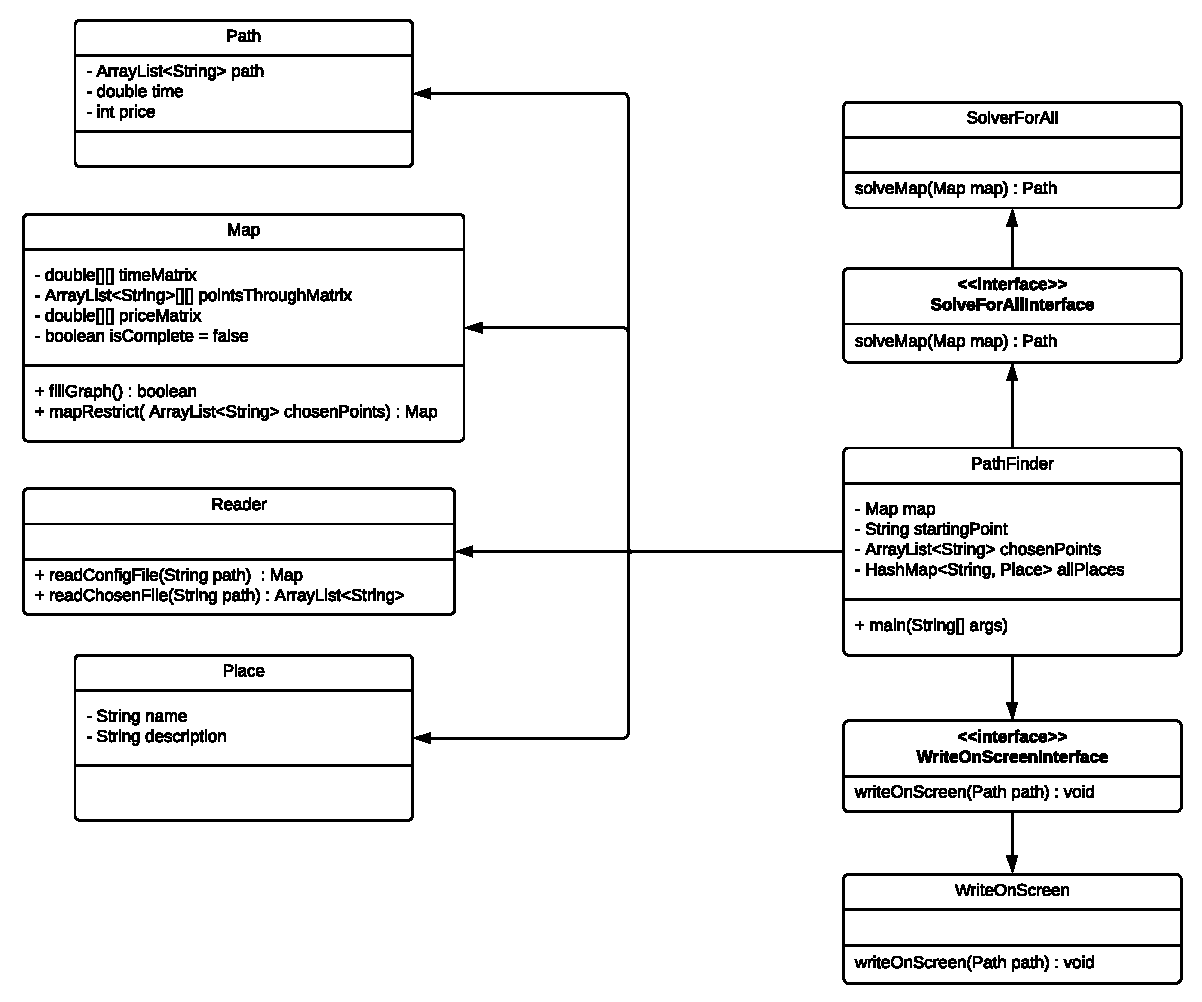
\includegraphics [height=9cm]{diagram_klas.pdf} \newline
\textit{Diagram klas ,,Bieszczadzki Komiwojażer''}

\subsection{Opis klas}
Przedstawienie funkcji i zadań poszczególnych klas.

\subsubsection{PathFinder}
Klasa głowna odpowiadająca za obsługiwanie programu. Przyjmuje argumenty wywołania, zarządza przebiegiem rozwiązania zadanego problemu i komunikacją z użytkownikiem.

\subsubsection{SolverForAll}
Klasa odpowiadająca za właściwe wyznaczenie rozwiązania. Wykorzystanie interfejsu umożliwia łatwą zmianę modułów i sposobów rozwiązywania problemu. Szczegółowy opis zastosowanych algorytmów znajduje się w części \textit{Schemat działania} i \textit{Algorytmy}.

\subsubsection{Path}
Klasa odpowiadająca za przechowywanie danych o rozwiązaniu. Pole \textit{path} to \textit{ArrayList<String>} zawierający następujące po sobie \textit{ID\_miejsca} trasy.

\subsubsection{Map}
Klasa odpowiadająca za przechowywanie danych o mapie. Zostaje wypełniona poprzez odczyt danych z pliku za pomocą klasy \textit{Reader}. Pole \textit{timeMatrix} to macierz incydencji otrzymanego grafu, którego wartości oznaczają czas przejścia pomiędzy konkretnymi wierzchołkami.

\subsubsection{Reader}
Klasa odpowiadająca za prawidłowe odczytanie danych z plików wejściowych oraz o odpowiednie zakomunikowanie o występujących w nich błędach. Metody \textit{readConfigFile()} i \textit{readChosenFile()} są odpowiedzialne za, odpowiednio, odczyt pliku konfiguracyjnego i odczyt pliku z wybranymi miejscami.

\subsubsection{Place}
Klasa przechowująca dane o miejscach odczytanych z pliku.

\subsubsection{WriteOnScreen}
Klasa przekazująca wynik końcowy użytkownikowi. Zastosowanie interfejsu umożliwi łatwą wymianę sposób komunikacji z użytkownikiem.

\subsection{Schemat działania}
Klasa \textit{PathFinder} rozpoczyna analizę argumentów wejściowych. Dokonuje odczytu podanych plików poprzez klasę \textit{Reader}. Następnie wywołuje metodę \textit{fillGraph()} klasy \textit{Map}, która, wykorzystując algorytm Djikstry, uzupełnia macierz incydencji tak, by opisywała graf pełny. Jeżeli został podany plik zawierający wybrane miejsca, wywołuje metodę \textit{mapRestrict()}, by ograniczyć graf tylko do miejsc, które mają być odwiedzone. Tak przygotowane zostają przekazane do funkcji \textit{solveMap()}. Otrzymany obiekt typu \textit{Path} zostaje przekazany do metody \textit{writeOnScreen} i przekazany użytkownikowi. 

\section{Algorytmy}
Podczas rozwiązywania zadanego problemu program będzie korzystał z implementacji następujących algorytmów.

\subsection{Algorytm Djikstry}
Algorytm służy do znajdowania najkrótszej możliwej drogi pomiędzy wybranym wierzchołkiem a pozostałymi wierzchołkami grafu. W programie zostanie wykorzystany, by dopełnić brakujące krawędzie grafu, zastępując je najkrótszą możliwą drogą wiodącą przez jak najmniejszą ilość innych punktów. 

Implementacja algorytmu wykorzystuje kolejkę priorytetową, w której priorytetem jest długość trwania trasy pomiędzy wierzchołkami. Idąc od wierzchołka początkowego, w każdej iteracji wybierany jest wierzchołek o najmniejszym koszcie. Jeżeli wierzchołek ma już określony koszt dotarcia, to wybierane jest minimum pomiędzy posiadaną wartością, a nową, ustaloną w bieżącym przebiegu algorytmu.

Złożoność czasowa algorytmu to O(E log V), gdzie E reprezentuje liczbę krawędzi, a V liczbę wierzchołków.

\subsection{Algorytm Helda-Karpa}
Algorytm służy do znajdowania minimalnego drzewa rozpinającego dla grafu pełnego. W programie zostanie wykorzystany do wyznaczenia najkrótszej możliwej drogi zawierającej wszystkie wierzchołki w grafie. Wzór algorytmu ma postać rekurencyjną i przedstawia się następująco:

    S -- zbiór wierzchołków grafu
    
    p należy do S -- wierzchołek grafu na którym ma zakończyć się droga
    
    D(S, p) -- najkrótsza możliwa droga z wybranego wierzchołka początkowego, przez wszystkie wierzchołki ze zbioru S, kończąca się na wierzchołku p.

    Jeśli s=1, to D(S, p) = d1,p,
    
    Jeśli s>1, to D(S, p) = min x należy do (S-{p})( D(S-{p}, x) + dx,p).

Jego złożoność czasowa wynosi O(n22n). Zapewnia dokładne wyznaczenie najkrótszej drogi przy złożoności mniejszej od O(n!).

\section{Struktury danych}
Program będzie wykorzystywał następujące struktury danych.

\subsection{Kopiec}
    Kopiec zostanie wykorzystany do implementacji kolejki priorytetowej, opisanej szczegółowo w sekcji \textit{Algorytm Djikstry}.
    
\subsection{Macierz}
    Macierz zostanie wykorzystana do przechowywania grafu w postaci macierzy incydencji, jak również kosztu przejścia i \textit{ID\_miejsca} wierzchołków przy uzupełnionym grafie.
    
\subsection{Tablica mieszająca}
    Tablica mieszająca (z ang. \textit{hash map}) zostanie wykorzystana do przechowywanie szczegółowych danych na temat punktów, jako klucz wykorzystując ich \textit{ID\_miejsca}.

\subsection{Lista liniowa}
    Lista liniowa w postaci \textit{ArrayList<>} zostanie wykorzystana do przechowywania listy wybranych miejsc.

\end{document}